\documentclass[12pt]{article}
\usepackage[spanish]{babel}

%%%%%%%%%%%%%%%%%%%%%%%%%%%%%%%%%%
%%%%%%%%%%%%%%%%%%%%%%%%%%%%%   %%
%%        Datos Trabajo     %%  %%
%%%%%%%%%%%%%%%%%%%%%%%%%%%%%%%%%%
\newcommand{\titulo}[0]{Tarea 3 \\ Algoritmos Elementales de Grafos}
\newcommand{\materia}[0]{AAeIMD}

\title{\titulo\\ \materia}
\author{Benjamin Rivera}
\date{\textit{Fecha de entrega:} \today}


%%%%%%%%%%%%%%%%%%%%%%%%%%%%%%%%%%
%%%%%%%%%%%%%%%%%%%%%%%%%%%%%%%%%%
\usepackage{amssymb}
\usepackage{enumerate}
\usepackage{geometry}
\usepackage{mathtools}
\usepackage{multicol}
\usepackage{soul}

\usepackage{graphicx}
	\graphicspath{ {assets/} }

\usepackage{hyperref}
	\hypersetup{
			pdftex,
		        pdfauthor={bench},
		        pdftitle={\titulo},
		        pdfsubject={\materia},
		        pdfkeywords={UG, bench},
		        pdfproducer={Latex with hyperref, Ubuntu},
		        pdfcreator={pdflatex, or other tool},
			colorlinks=true,
				linkcolor=[rgb]{0,0,0.45},
				urlcolor=cyan,
				filecolor=green,
				citecolor=blue}
    
\begin{document}

\maketitle

\noindent
\textbf{Ejercicio 1}. Dibuje un grafo no-dirigido conectado tal que cada vértice esté en algún ciclo no dirigido, pero que independientemente de la orientación que se de a las aristas (es decir que se conviertan en aristas dirigidas) el grafo no esté fuertemente conectado.

\par \textbf{Respuesta}




\begin{figure}[h]
	\centering
	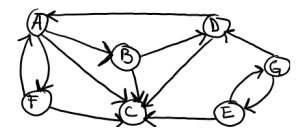
\includegraphics[width=0.4\textwidth]{grafo1.png}
	\caption{Grafo 1}
	\label{fig: 1}
\end{figure}






\par\ \\\ \\\noindent
\textbf{Ejercicio 2}. Determine los árboles de búsqueda primero en profundidad (DFS) para el
grafo de la Figura 1 con G como vértice de partida y haciendo el siguiente supuesto acerca
del orden dentro de las listas de adyacencia:
\begin{itemize}
	\item Cada lista de adyacencia está en orden alfabético.
\end{itemize}

\textbf{Nota:} En el diagrama del árbol de búsqueda, muestre el tiempo (paso) en el que se descubrió y terminó cada elemento. Por ejemplo, 4/7 indica que se descubrió en el 4 y se terminó en 7.

\par \textbf{Respuesta}





\par\ \\\ \\\noindent
\textbf{Ejercicio 3}. Determine el árbol de búsqueda primero en profundidad (DFS) para el grafo de la Figura 1 con G como vértice de partida y haciendo el siguiente supuesto acerca del orden dentro de las listas de adyacencia:
\begin{itemize}
	\item Cada lista de adyacencia está en orden alfabético inverso.
\end{itemize}

\textbf{Nota:} En el diagrama del árbol de búsqueda, muestre el tiempo (paso) en el que se
descubrió y terminó cada elemento. Por ejemplo, 4/7 indica que se descubrió en el 4 y se
terminó en 7.

\par \textbf{Respuesta}






\par\ \\\ \\\noindent
\textbf{Ejercicio 4}. Sea G un grafo conectado, y sea s un vértice de G. Sea $T_D$ un árbol de búsqueda DFS que se forma efectuando una búsqueda primero en profundidad en G partiendo de s. Sea $T_B$ un árbol abarcante primero en en amplitud (BFS) que se forma efec tuando búsqueda primero en amplitud en G partiendo de s. ¿Siempre se cumple que $altura(T_D ) \leq altura(T_B )$ ?¿Importa si el grafo es dirigido o no? Presente un argumento claro o un contraejemplo.

\par \textbf{Respuesta}







\par\ \\\ \\\noindent
\textbf{Ejercicio 5}. Ejecute rastreo DFS con el grafo dirigido de la Figura 2, y clasifique todas las aristas. Para esta clasificación redibuje el grafo que muestre los tiempos de descubrimiento y terminación de cada elemento explorado (igual que en la nota del Ejercicio 2). En su nuevo diagrama utilice la siguiente notación para etiquetar las aristas: (t) tree edge, (b) back edge, (c) cross edge y (f) forward edge. Para este ejercicio suponga que los vértices están indexados en orden alfabético en un arreglo vertices Adya y que todas las listas de adyacencia están en {\Large\bf orden alfabético.}

\par \textbf{Respuesta}





\begin{figure}[h]
	\centering
	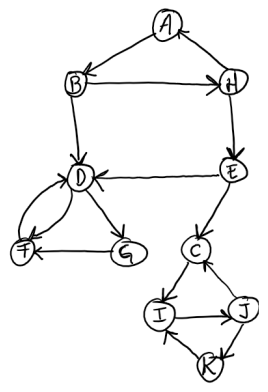
\includegraphics[width=0.3\textwidth]{grafo2.png}
	\caption{Grafo 1}
	\label{fig: 1}
\end{figure}








\par\ \\\ \\\noindent
\textbf{Ejercicio 6}. Ejecute rastreo DFS con el grafo dirigido de la Figura 2, y clasifique todas las aristas. Para esta clasificación redibuje el grafo que muestre los tiempos de descubrimiento y terminación de cada elemento explorado (igual que en la nota del Problema 2). En su nuevo diagrama utilice la siguiente notación para etiquetar las aristas: (t) tree edge, (b)
back edge, (c) cross edge y (f) forward edge. Para este ejercicio suponga que los vértices
están indexados en orden alfabético inverso en un arreglo verticesAdya y que todas las listas
de adyacencia están en {\Large\bf orden alfabético inverso.}

\par \textbf{Respuesta}






\par\ \\\ \\\noindent
\textbf{Ejercicio 7}. Suponga que quiere hallar un camino más corto de $s$ a $w$ en un grafo $G$ en el que la longitud de cualquier camino es simplemente el número de aristas del camino (por ejemplo, planear un viaje en avión con el m\'inimo de escalas). Explique detalladamente qué estrategia(s)/algoritmo(s) representa(n) la mejor alternativa a este problema y ¿por qué?.

\par \textbf{Respuesta}






\par\ \\\ \\\noindent
\textbf{Ejercicio 8}. De un ejemplo de algún grafo dirigido $G = (V, E)$, un vértice de inicio $s \in V$ , y un conjunto de aristas de árbol $E_\pi \subseteq E$ tal que para cada vértice $v \in V$ , el único camino simple en el grafo $V, E_\Pi$ de $s$ a $v$ es el camino más corto en G. En este ejemplo, el conjunto de aristas $E_\pi$ debe ser imposible de generar con BFS ejecutado sobre G, sin importar el orden de los vértices en la lista de adyacencia.

\par \textbf{Respuesta}






\par\ \\\ \\\noindent
\textbf{Ejercicio 9}. Si un grafo dirigido $G$ contiene un camino de $u$ a $v$, entonces $u (u.d)$ se descubre siempre antes de $v (v.d)$ en un BFS del grafo $G$, y por lo tanto v es un descendiente de $u$ en el DFS forest que se produce. Lo anterior, ¿siempre se cumple? Presente un argumento claro del porque o un contraejemplo. 

\par \textbf{Respuesta}





\end{document}

